\documentclass[
  captions=tableheading,
  bibliography=totoc, 
  titepage=firstiscover,
]{scrartcl}

\usepackage{blindtext} %neuer input

\usepackage{longtable} % Tabellen über mehrere Seiten

\usepackage[utf8]{inputenc} %neuer input

\usepackage{scrhack}

\usepackage[aux]{rerunfilecheck} %Warnung falls nochmal kompiliert werden muss

\usepackage{fontspec} %Fonteinstellungen

\recalctypearea{}

\usepackage[main=ngerman]{babel} %deutsche Spracheinstellung

\usepackage{ragged2e} %neuer input

\usepackage{amsmath, nccmath}

\usepackage{amssymb} %viele mathe Symbole

\usepackage{mathtools} %Erweiterungen für amsmath


\DeclarePairedDelimiter{\abs}{\lvert}{\rvert}
\DeclarePairedDelimiter{\norm}{\lVert}{\rVert}

\DeclarePairedDelimiter{\bra}{\langle}{\rvert}
\DeclarePairedDelimiter{\ket}{\lvert}{\rangle}

\DeclarePairedDelimiterX{\braket}[2]{\langle}{\rangle}{
#1 \delimsize| #2
}

\NewDocumentCommand \dif {m}
{
\mathinner{\symup{d} #1}
}


\usepackage[
  math-style=ISO,
  bold-style=ISO,
  sans-style=italic,
  nabla=upright,
  partial=upright,
  warnings-off={
    mathtools-colon,
    mathtools-overbracket,
  },
]{unicode-math}

\setmathfont{Latin Modern Math}
\setmathfont{XITS Math}[range={scr, bfscr}]
\setmathfont{XITS Math}[range={cal, bfcal}, StylisticSet=1]


\usepackage[
  locale=DE,
  separate-uncertainty=true,
  per-mode=reciprocal,
  output-decimal-marker={,},
]{siunitx}

\usepackage[autostyle]{csquotes} %richtige Anführungszeichen

\usepackage{xfrac}

\usepackage{float}

\floatplacement{figure}{htbp}

\floatplacement{table}{htbp}

\usepackage[ %floats innerhalb einer section halten
  section,   %floats innerhalb er section halten
  below,     %unterhalb der Section aber auf der selben Seite ist ok
]{placeins}

\usepackage[
  labelfont=bf,
  font=small,
  width=0.9\textwidth,
]{caption}

\usepackage{subcaption} %subfigure, subtable, subref

\usepackage{graphicx}

\usepackage{grffile}

\usepackage{booktabs}

\usepackage{microtype} %Verbesserungen am Schriftbild

\usepackage[
backend=biber,
]{biblatex}

\addbibresource{../lit.bib}

\usepackage[ %Hyperlinks im Dokument
  german,
  unicode,
  pdfusetitle,
  pdfcreator={},
  pdfproducer={},
]{hyperref}

\usepackage{bookmark}

\usepackage[shortcuts]{extdash}

%\usepackage{warpcol}

\allowdisplaybreaks

\begin{document}
    \title{Physik IV Übungsblatt 5}
    \author{  
    Tobias Rücker\\
    \texorpdfstring{\href{mailto:tobias.ruecker@tu-dortmund.de}{tobias.ruecker@tu-dortmund.de}
    \and}{,} 
    Paul Störbrock\\
    \texorpdfstring{\href{mailto:paul.stoerbrock@tu-dortmund.de}{paul.stoerbrock@tu-dortmund.de}}{}
    }
\maketitle
\center{\Large Abgabegruppe: \textbf{4H}}
\thispagestyle{empty}

\newpage
\tableofcontents
\thispagestyle{empty}
\newpage

\setcounter{page}{1}

\section{Aufagabe 1}

    \begin{figure}[H]
        \centering
        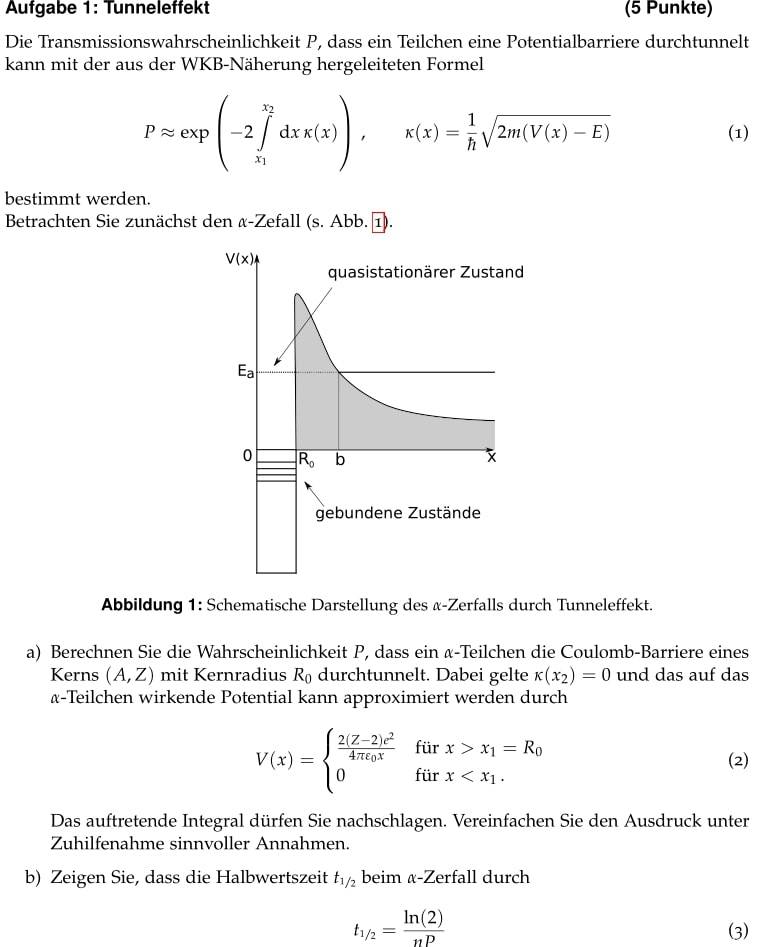
\includegraphics[width=\textwidth]{images/Aufgabe1a.jpg}
        \label{fig:1}
    \end{figure}
        \begin{figure}[H]
        \centering
        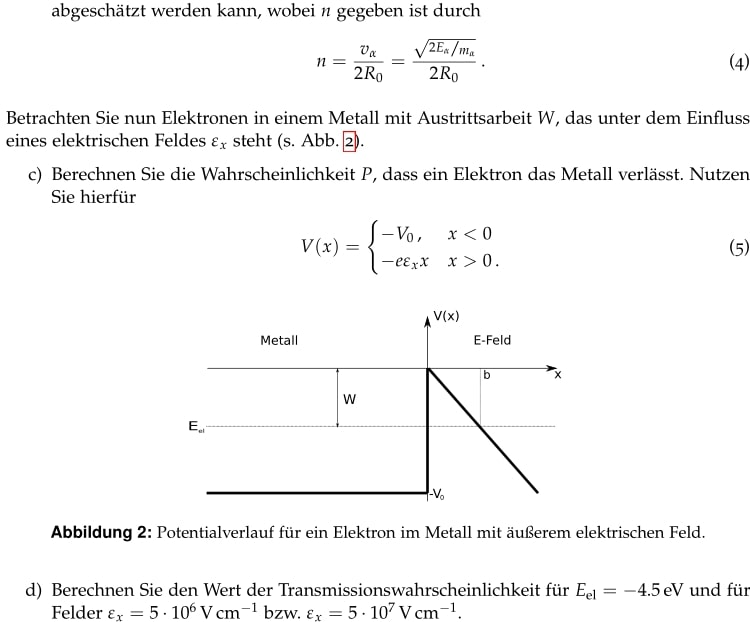
\includegraphics[width=\textwidth]{images/Aufgabe1bcd.jpg}
        \label{fig:2}
    \end{figure}

\subsection{a)}

    \begin{align*}
        P &\approx exp\left(-2 \int_{x_1}^{x_2} \mathrm{d}x \, \kappa(x)\right)\\
        \kappa(x) &= \frac{1}{\hbar} \sqrt{2m(V(x)-E)} \tag{*}
        \intertext{\flushleft{Potential\;}\justifying des $\alpha$-Teilchens:
        }
        V(x)
        &\begin{cases}
            \frac{2(z-2)e^2}{4\pi \epsilon_0 x} \qquad \text{für}\; x > x_1=R_0 \qquad \text{einsetzten in (*)}\\
            0 \qquad \qquad \quad \!\text{für}\; x<x_1
        \end{cases}
        \intertext{\flushleft{Die\;}\justifying Wahrscheinlichkeit $P$, mit der das $\alpha$-Teilchen die Potentialbarriere durchtunnelt:
        }
        P(x) &\approx exp\left( -2 \int_{R_0}^{b} \frac{1}{\hbar} \sqrt{2m\left( \frac{2(z-2)e^2}{4\pi \epsilon_0 x} -E \right)} \mathrm{d}x \right)
        \intertext{\flushleft{Substitution:\;}\justifying
        }
        b &= \frac{2(z-2)e^2}{4\pi \epsilon_0 E}\\
        \frac{x}{b} &= \sin^2(u) \Leftrightarrow x = b\sin^2(u) \Leftrightarrow \frac{b}{x} = \frac{1}{\sin^2(u)}\\
        \frac{\mathrm{d}x}{\mathrm{d}u} &= 2b \sin(u)\cos(u)\\
        \Leftrightarrow \mathrm{d}x &= 2b \sin(u)\cos(u) \mathrm{d}u
        \intertext{\flushleft{Für\;}\justifying $\mathrm{d}u$ und $b$ substituieren: (Es werden nur die Terme im Exponenten betrachtet)
        }
    	&= -2 \int_{u(R_0)}^{u(b)} 2b \frac{\sqrt{2mE}}{\hbar}\sin(u)\cos(u) \underbrace{\sqrt{\frac{1}{\sin^2(u)}-1}}_{=\cot(u)} \,\mathrm{d}u\\
        &= -4 \int_{u(R_0)}^{u(b)} \frac{b}{\hbar}\,\sqrt{2mE}\, \sin(u)\cos(u) \cot(u)\,\mathrm{d}u\\
        &= -4 \int_{u(R_0)}^{u(b)} \frac{b}{\hbar}\,\sqrt{2mE}\, \cos^2(u)\, \mathrm{d}u\\
        &= -4 \frac{b}{\hbar}\sqrt{2mE}\, \left[ \frac{1}{2} \left( u+\sin(u)\cos(u) \right) \right]_{u(R_0)}^{u(b)}\\
        &= -2 \frac{b}{\hbar}\sqrt{2mE}\, (u(b)+\sin(u(b))\cos(u(b)))-u(R_0)-\sin(u(R_0))\cos(u(R_0))
        \intertext{\flushleft{Die\;}\justifying Grenzen in $u$ einsetzten:
        }
        u &= \arcsin\left(\sqrt{\frac{x}{b}}\right)\\
        u(b) &= \arcsin\left(\sqrt{\frac{b}{b}}\right) = \frac{\pi}{2}\\
        u(R_0) &= \arcsin\left(\sqrt{\frac{R_0}{b}}\right)
        \intertext{\flushleft{$u$\;}\justifying resubstituieren:
        }
        &= -2 \frac{b}{\hbar}\sqrt{2mE}\, \left(\frac{\pi}{2}-\arcsin\left(\sqrt{\frac{R_0}{b}}\right)-\sqrt{\frac{R_0}{b}} \cos\left(\arcsin(\sqrt{\frac{R_0}{b}}\right)\right)\\
        &= -2 \frac{b}{\hbar}\sqrt{2mE}\, \left(\frac{\pi}{2}-\arcsin\left(\sqrt{\frac{R_0}{b}}\right)-\sqrt{\frac{R_0}{b}} \sqrt{1-\frac{R_0}{b}} \right)
        \intertext{\flushleft{Für\;}\justifying $\frac{R_0}{b} \ll 1 \to \arcsin(x) \approx x$:
        }
        &= -2 \frac{b}{\hbar}\sqrt{2mE}\, \left(\frac{\pi}{2}-2\sqrt{\frac{R_0}{b}} \right)\\
        \Rightarrow P &\approx exp\left(-2 \frac{b}{\hbar}\sqrt{2mE}\, \left(\frac{\pi}{2}-2\sqrt{\frac{R_0}{b}} \right)\right)
    \end{align*}

\subsection{b)}

    \begin{align*}
        \intertext{\flushleft{Beim\;}\justifying Alpha Zerfall wird angenommen, dass das Alpha-Teilchen gegen die Wände 
        des Atomkerns stößt. Seine Stoßzeit lässt sich dann berechnen durch:
        }
        t_0 &= \frac{2R}{v} \tag{*}\\
        E &\approx \frac{1}{2}mv^2 \Leftrightarrow v \approx \sqrt{\frac{2E}{m}}
        \intertext{\flushleft{Die\;}\justifying Lebensdauer des Atoms entspricht im Mittel dann der Stoßzeit geteilt durch die 
        Transmissionswahrscheinlichkeit.
        }
        \tau &\approx \frac{t_0}{P}
        \stackrel{(*)}{=} \frac{1}{nP}
        \intertext{\flushleft{In\;}\justifying der Zeit $\mathrm{d}t$ zerfällen dN  Kerne in der Zeit dt.
        Die Wahrscheinlichkeit, das ein Kern im Zeitintervall zerfällt, ist durch $\sfrac{dt}{\tau} $ gegeben.
        }
        \mathrm{d}N &= -\frac{N}{\tau} \mathrm{d}t
        \intertext{\flushleft{Die:\;}\justifying Lösung der DGL ergibt:
        }
        N &= N_0 exp\left( -\frac{t}{\tau} \right)\\
        \frac{N}{N_0} &= \frac{1}{2} = exp\left( -\frac{t_{\sfrac{1}{2}}}{\tau} \right)\\
        \ln\left( \frac{1}{2}\right) &= -\frac{t_{\sfrac{1}{2}}}{\tau}\\
        -\ln(2) \tau &= -t_{\sfrac{1}{2}} \qquad \left( \tau = \frac{1}{nP} \right)\\
        t_{\sfrac{1}{2}} &= \frac{\ln(2)}{nP}
    \end{align*}

\subsection{c)}

    \begin{align*}
        V(x)
        &\begin{cases}
            -V_0, \qquad x<0\\
            -e\epsilon_x x, \quad x>0
        \end{cases}\\
        P(x) &= exp\left( -2 \int_{0}^{b} \kappa(x) \mathrm{d}x \right)\\
        &= exp\left( -2 \int_{0}^{b} \frac{1}{\hbar} \sqrt{2m(-e\epsilon_x x-E)}\, \mathrm{d}x \right)
        \intertext{\flushleft{$2mE$\;}\justifying ausklammern:
        }
        &= exp\left( -2 \frac{\sqrt{2mE}}{\hbar} \int_{0}^{b} \sqrt{-\frac{e\epsilon_x x}{E}-1}\, \mathrm{d}x \right)
        \intertext{\flushleft{Substitution:\;}\justifying
        }
        u &= -\frac{e\epsilon_x x}{E}-1\\
        \frac{\mathrm{d}u}{\mathrm{d}x} &=  -\frac{e\epsilon_x}{E}\\
        \Leftrightarrow \mathrm{d}x &= \frac{-E}{e\epsilon_x}\, \mathrm{d}u
        \intertext{\flushleft{$u$\;}\justifying und $\mathrm{d}x$ einsetzten:
        }
        &= exp\left( -2 \frac{\sqrt{2mE}}{\hbar} \int_{-1}^{u(b)} \sqrt{u} \frac{(-E)}{e\epsilon_x}\, \mathrm{d}u \right)\\
        &= exp\left( 2 \frac{\sqrt{2mE^3}}{\hbar e\epsilon_x} \left[ \frac{2}{3} u^{\frac{3}{2}} \right]_{-1}^{u(b)} \right)
        \intertext{\flushleft{$u$\;}\justifying rücksubstituieren:
        }
        &= exp\left( \frac{4}{3} \frac{\sqrt{2mE^3}}{\hbar e\epsilon_x} \left( \sqrt{\left( -\frac{e\epsilon_x b}{E}-1 \right)^3}-\sqrt{-1} \right) \right)\\
        E_{el} &= -e\epsilon_x b\\
        \Leftrightarrow b &= -\frac{E_{el}}{e\epsilon_x}
        \intertext{\flushleft{$b$\;}\justifying einsetzten:
        }
        &= exp\left( \frac{4}{3} \frac{\sqrt{2mE^3}}{\hbar e\epsilon_x} \left( \sqrt{1-1}-\sqrt{-1} \right) \right)\\
        &= exp\left( -\frac{4}{3} \frac{\sqrt{-2mE^3}}{\hbar e\epsilon_x} \right)
    \end{align*}

\subsection{d)}

    \begin{align*}
        \intertext{\flushleft{$P$\;}\justifying für $E_{el}=-4.5eV$ und $\epsilon_x=\SI{5e+08}{\volt\per\meter}$:
        }
        P_1 = exp\left( -\frac{4}{3} \frac{\sqrt{ -2m_e \cdot \SI{-91.125}{\electronvolt}}}{\hbar e \cdot \SI{5e+08}{\volt\per\meter}} \right) = \text{\input{P_1.tex}}
        \intertext{\flushleft{$P$\;}\justifying für $E_{el}=-4.5eV$ und $\epsilon_x=\SI{5e+09}{\volt\per\meter}$:
        }
        P_2 = exp\left( -\frac{4}{3} \frac{\sqrt{ -2m_e \cdot \SI{-91.125}{\electronvolt}}}{\hbar e \cdot \SI{5e+09}{\volt\per\meter}} \right) = \text{\input{P_2.tex}}
    \end{align*}

\section{Aufgabe 2}

    \begin{figure}[H]
        \centering
        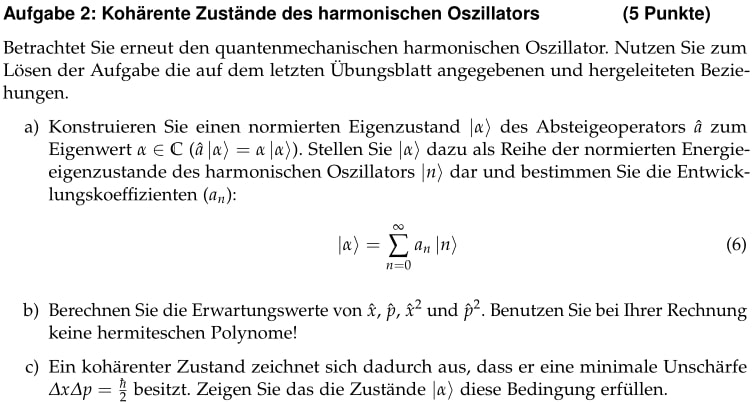
\includegraphics[width=\textwidth]{images/Aufgabe2abc.jpg}
        \label{fig:3}
    \end{figure}
    \begin{figure}[H]
        \centering
        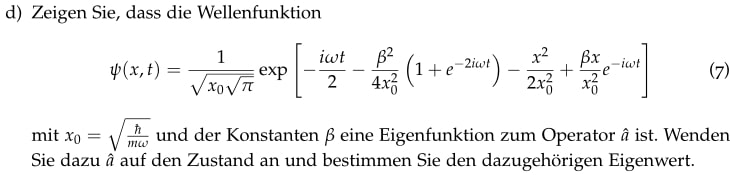
\includegraphics[width=\textwidth]{images/Aufgabe2d.jpg}
        \label{fig:4}
    \end{figure}

\subsection{a)}

\subsection{b)}

\subsection{c)}

\subsection{d)}


\section{Aufgabe 3}

    \begin{figure}[H]
        \centering
        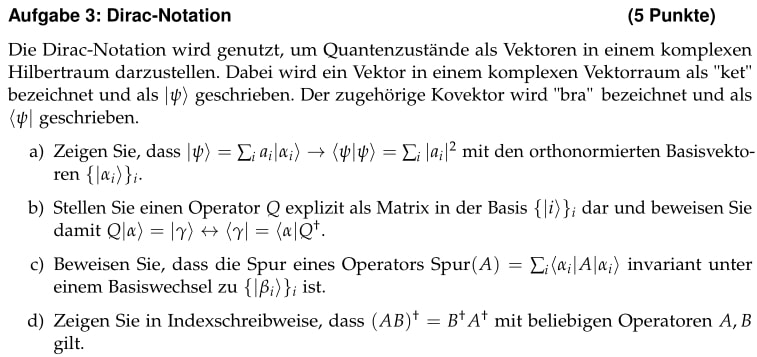
\includegraphics[width=\textwidth]{images/Aufgabe3.jpg}
        \label{fig:5}
    \end{figure}

\subsection{a)}

    \begin{align*}
        \vert \alpha_i \rangle &= 
        \begin{pmatrix}
            \alpha_1\\
            \alpha_2\\
            \vdots\\
            \alpha_n
        \end{pmatrix} \qquad
        \langle \alpha_i \vert =
        \begin{pmatrix}
            \alpha_1^*, & \alpha_2^*, & \ldots, & \alpha_n^*
        \end{pmatrix}\\
        \vert \psi \rangle &= \sum_{i} a_i \vert \alpha_i \rangle = a_1 \alpha_1 + a_2 \alpha_2 + \ldots + a_n \alpha_n\\
        \langle \psi \vert &= \sum_{i} \langle \alpha_i \vert a_i = a_1 \alpha_1^* + a_2 \alpha_2^* + \ldots + a_n \alpha_n^*\\
        \langle \psi \vert \psi \rangle &= \sum_{i} \langle \alpha_i \vert a_i \cdot a_i \vert \alpha_i \rangle 
        = \sum_{i} a_i^2 \underbrace{\langle \alpha_i \vert \alpha_i \rangle}_{ONB \Rightarrow =1}\\
        &= \sum_{i} a_i^2 \Leftrightarrow \sum_{i} \vert a_i \vert^2
    \end{align*}

\subsection{b)}

    \begin{align*}
        Q &=
        \begin{pmatrix}
        q_{11} & q_{12} & \ldots & q_{1n}\\
        q_{21} & q_{22} & \ldots & q_{2n}\\
        \vdots & \vdots & \ddots & \vdots\\
        q_{m1} & q_{m2} & \ldots & q_{mn}
        \end{pmatrix}\\
        Q \vert \alpha_i \rangle &=
        \begin{pmatrix}
        q_{11} & q_{12} & \ldots & q_{1n}\\
        q_{21} & q_{22} & \ldots & q_{2n}\\
        \vdots & \vdots & \ddots & \vdots\\
        q_{m1} & q_{m2} & \ldots & q_{mn}
        \end{pmatrix} \cdot 
        \begin{pmatrix}
            \alpha_1\\
            \alpha_2\\
            \vdots\\
            \alpha_n
        \end{pmatrix}\\
        &= \sum_{i} \alpha_i \sum_{j} q_{ij} = \vert \gamma \rangle\\
        \langle \alpha_i \vert Q^{\dagger} &=
        \begin{pmatrix}
            \alpha_1^*, & \alpha_2^*, & \ldots, & \alpha_n^*
        \end{pmatrix} \cdot 
        \begin{pmatrix}
        q_{11}^* & q_{21}^* & \ldots & q_{m1}^*\\
        q_{12}^* & q_{22}^* & \ldots & q_{m2}^*\\
        \vdots & \vdots & \ddots & \vdots\\
        q_{1n}^* & q_{2n}^* & \ldots & q_{nm}^*
        \end{pmatrix}\\
        &= \sum_{i} \alpha_i^* \sum_{j} q_{ji}^* = \langle \gamma \vert
    \end{align*}

\subsection{c)}

    \begin{align*}
        \text{Spur}(A) &= \sum_{i} \langle \alpha_i \vert A \vert \alpha_i \rangle \qquad \text{mit Basisvektor}\; \vert \beta_i \rangle
        \intertext{\flushleft{Erweitern\;}\justifying um $\vert \beta_j \rangle \cdot \langle \beta_j \vert=1$ und $\vert \beta_k \rangle \cdot \langle \beta_k \vert=1$:
        }
        &= \sum_{i} \sum_{j,k} \langle \alpha_i \vert \beta_j \rangle \langle \beta_j \vert A \vert \beta_k \rangle \langle \beta_k \vert \alpha_i \rangle
        \intertext{{Durch\;}\justifying Umstellen (Sortieren) können die $\alpha_i$ zusammengefasst werden:
        }
        &= \sum_{j,k} \langle \beta_k \vert \underbrace{\left( \sum_{i} \vert \alpha_i \rangle \cdot \langle \alpha_i \vert \right)}_{=1\;(Einheitsoperator)} \vert \beta_j \rangle \langle \beta_j \vert A \vert \beta_k \rangle\\
        &= \sum_{j,k} \langle \beta_k \vert \beta_j \rangle \langle \beta_j \vert A \vert \beta_k \rangle\\
        \langle \beta_k \vert \beta_j \rangle
        &\begin{cases}
            1 \qquad \text{für}\; j=k\\
            0 \qquad \text{sonst}
        \end{cases}\\
        \Rightarrow \delta_{jk} &= \langle \beta_k \vert \beta_j \rangle
        \intertext{\flushleft{Da\;}\justifying die Spur$(A)$ nur $\neq 0$ ist für j=k folgt:
        }
        \text{Spur}(A) &=\sum_{j,k} \delta_{jk} \langle \beta_j \vert A \vert \beta_k \rangle = \sum_{k} \langle \beta_k \vert A \vert \beta_k \rangle
    \end{align*}

\subsection{d)}


\end{document}